\documentclass[twocolumn,conference]{IEEEtran}
\usepackage[T1]{fontenc}
\usepackage[latin9]{inputenc}
\usepackage{url}
\usepackage{graphicx, import, xcolor}
\usepackage{soul}
\usepackage{multirow}
\renewcommand\IEEEkeywordsname{Keywords}
\usepackage{amsmath}
\usepackage{cases}
\usepackage{makecell}
\usepackage[section]{placeins}
\usepackage{subcaption}
\usepackage{mathtools}
\DeclarePairedDelimiter\abs{\lvert}{\rvert}
\newcolumntype{C}[1]{>{\centering\let\newline\\\arraybackslash\hspace{0pt}}m{#1}}
\newcolumntype{R}[1]{>{\raggedleft\let\newline\\\arraybackslash\hspace{0pt}}m{#1}}
\makeatletter
\DeclareRobustCommand{\textsupsub}[2]{{%
  \m@th\ensuremath{%
    ^{\mbox{\fontsize\sf@size\z@#1}}%
    _{\mbox{\fontsize\sf@size\z@#2}}%
  }%
}}
\makeatother

\begin{document}
\title{Circuits to Access Resistive Memories with High State Capacity}
%\author{
%      Thanasin Bunnam,
%      Oleg Mayevsky,
%      Ahmed Soltan,
%      Danil Sokolov,
%      Alex Yakovlev\\
%      School of Electrical and Electronic Engineering, Newcastle University, UK
% }

\maketitle

\begin{abstract}
Metastability is a special consideration in many emerging memory technologies. This paper discusses trade-offs and optimizations that involve metastable behavior in a memristor-based memory. Following our prior experience in handling metastability in A-to-D converters, we propose a new method for designing a mechanism to read a memristor with high state capacity. The method uses an accurate sense amplifier with metastability resolution and completion detection, and shows robustness against PVT variations due to the use of reference resistor set with resistive buffers. Furthermore, the single supply voltage requirement is the outstanding feature among the available research works.  For demonstration of the proof of concept, a 2-bit memristor-based multi-bits memory cell (3MCell) has been built. It consists of four components: resistance comparator, reference resistor set, memristor and interface, and controllers which are built in synchronous and asynchronous versions. Simulation results support our extensive validation of the proposed circuits.

\end{abstract}

\begin{IEEEkeywords}
memristor, multi-bits memory, resistance comparator, metastability, memory controller
\end{IEEEkeywords}

\section{Introduction}
\label{sec:introduction}
Memristor was introduced in 1971 as a missing element that links charge and flux~\cite{Chua-1971-TCT}. Implementations were later investigated with a first successful practical device appearing in 2008~\cite{Strukov-2008-Nature}. Since that time, many challenges have been explored, such as: fast switching, small footprint, high energy efficiency and CMOS process compatibility~\cite{Vourkas-2016-MCAS} ~\cite{Vourkas-2016-Springer} ~\cite{Sacchetto-2013-MCAS}.

The key feature that makes it an outstanding device for ``beyond CMOS'' computing is the adjustable internal resistance (memristance) that keeps its value without power, thus lending itself to non-volatile memory. This feature broadens research frontiers, such as neural networks, neuromorphic system~\cite{Vourkas-2016-MCAS}~\cite{Tetzlaff-2014-Springer} and self-adaptive timing circuit~\cite{Gu-2015-ISCAS}~\cite{Bunnam-2017-PATMOS}.
Moreover, the memristor supports higher endurance than NAND flash~\cite{ITRS-2015}~\cite{Yang-2013-Nature} and long data retention~\cite{Tetzlaff-2014-Springer}~\cite{ITRS-2015}. Therefore, it is considered as a promising device for the future memory cell.

Regarding the highlighted feature, today, there are many research attempts to build a memristor-based memory. They can be classified into two categories: digital~\cite{Emara-2014-CEEC}~\cite{Elshamy-2015-TVLSI} and analog (multi-bits) memories~\cite{Emara-2014-CEEC}~\cite{Manem-2011-ISCAS}~\cite{Soell-2017-CTA}~\cite{Wang-2017-TCAD}~\cite{Yilmaz-2017-TNano}. The concept of digital memory is to switch the memristance between low and high values (low and high resistive states in the literature) to represent binary logic (0 and 1) while the latter improves the utilization and data density by sectioning the memristance range into small pieces and allotting each piece to a datum. In this way, multiple bits of data can be stored in only one memristor and, consequently, the area and power consumption may be reduced.

Previously proposed memristor-based multi-bit memories been designed equipped with switching devices and multiple supply voltages to avoid sneak paths that cause neighbor tuning and power loss~\cite{Emara-2014-CEEC}~\cite{Manem-2011-ISCAS}~\cite{Soell-2017-CTA}~\cite{Wang-2017-TCAD}~\cite{Yilmaz-2017-TNano}. However, using multi-voltages supply requires voltage regulation circuits and increases overall circuit complexity.

A comparator is needed for reading data from this kind of memory -- it can distinguish between the memristor voltage, which reflects the memristance, and the reference one. The precision of the comparator defines the data resolution and capacity. However, the widely used amplifier-based comparator suffers from noise because it amplifies both the unwanted signal and the original one.

This paper presents a new ways to designing memristor-based multi-bits memory cell (3MCell). The advantages of this design are as follows: a single supply voltage, high data capacity support and PVT variation tolerance. Single supply voltage is supported by the proposed \textit{resistance comparator}, which permits a small voltage drop at the memristor terminal so that it cannot shift the memristance. Our resistance comparator design operates at high precision to provide a high data capacity. Besides, it can be considered as noise-tolerant due to a non-amplifier based design. This paper also shows a solution for the metastability that the comparator enters when the resistances under comparison are close. To improve robustness to PVT variations, the reference resistor set (RSet) is designed to provide resistive buffers between data regions. Finally, the controller is also developed in both synchronous and asynchronous scheme.

This work uses VTEAM memristor model~\cite{Kvatinsky-2015-TCSII}, which is a threshold-based voltage-driven model, because it is compatible with the other models and it can be flexibly fitted with most of practical devices as well as the newly invented ones. All circuits and simulations are based on UMC 65nm Low Leakage technology.
\section{System Overview}
\label{sec:SystemOverview}
\subsection{Data Representation}
\label{subsec:DataRepresentation}
Based on the selected CMOS technology, the operating voltage of the MOSFET is 1.2V. Regarding VTEAM model parameters, the threshold voltages (v\textsubscript{on} and v\textsubscript{off}) must be lower than the operating voltage to allow the memristance shift. Unfortunately, to the best of our knowledge, there is no  VTEAM parameter sets that meet this condition. Therefore, the parameter set with the closest threshold voltages (v\textsubscript{on}=-1.5V)~\cite{Kvatinsky-2014-TCSII} is modified as listed in Table~\ref{tab:MemristorFittingParameters} while v\textsubscript{off} is untouched because it already meets the condition. Moreover, k\textsubscript{on} and k\textsubscript{off} are also adjusted to slow down the memristance shifting speed and to guarantee the over-shift, where an amount of memristance shift is larger than one data region, does not occur with the given tuning time (10ns). Note that the memristor with these modified properties can be achieved by device sizing~\cite{Li-2015-ISCAS}.
\begin{table}[ht]
   \centering
   \caption{VTEAM Fitting Parameters.}
   \label{tab:MemristorFittingParameters}
   \begin{tabular}{| l | r | l |}
       \hline
       \thead{Parameter}& 
       \thead{Value}&
       \thead{Unit}\\
       \hline
       \hline
       $\alpha$\textsubscript{off}    &  4  & $-$ \\
	   \hline
	   $\alpha$\textsubscript{on}    &  4  & $-$	\\
       \hline
       v\textsubscript{off}  	&  0.3  & V \\
       \hline
       v\textsubscript{on}		&  -1.0 & V	\\
       \hline
       R\textsubscript{off}	&  300K & $\Omega$ \\
       \hline
       R\textsubscript{on}		&  1K 	& $\Omega$ \\
       \hline
       k\textsubscript{off}	&  $250\times10^{-6}$ & m/s \\
       \hline
       k\textsubscript{on} 	&  -7	& m/s \\
       \hline
       D			&  3	& nm \\
       \hline
%        ON to OFF switching time & \multirow{2}{*}{148.14} & \multirow{2}{*}{ns} \\
%        (1.2V biasing voltage) & & \\
%        \hline
%        OFF to ON switching time & \multirow{2}{*}{267.85} & \multirow{2}{*}{ns} \\
%        (1.2V biasing voltage) & & \\
%        \hline
   \end{tabular}
\end{table}
From Table~\ref{tab:MemristorFittingParameters}, it can be seen that there is a memristance range of 299K$\Omega$ which is large enough for division to represent 4 data. However, the memristance range in the middle (120K$\Omega$-180K$\Omega$) is preferred to ensure better linearity. The latter is affected by the window effect when the memristance is shifted near to the device boundary either R\textsubscript{on} or R\textsubscript{off}. 

Also, it can be seen that ON-to-OFF threshold (v\textsubscript{off}) is very low, hence, connecting this side close to ground is preferred as it guarantees the voltage drop will not exceed the threshold. By this assumption, OFF-to-ON (v\textsubscript{on}) side is turned to the comparator and 2-bits data 00 to 11 is arranged in R\textsubscript{off} to R\textsubscript{on} direction. To avoid confusion as ``low'' value data is represented by ``high'' resistance and vice versa, this paper presents data in term of conductance instead. Therefore, low value data is represented by low conductance.

In addition, to prevent the unexpected memristance shift due to PVT variations, the resistive ``buffers'' have been added between each data region. In this work, each data region and buffer contains a memristance range of 14K$\Omega$ and 6K$\Omega$, respectively. Table~\ref{tab:DataRepresentation} summarizes the data representation in this work. Note that G\textsubscript{min}=1/R\textsubscript{off} and G\textsubscript{max} is assumed as $\infty$ (wire).
\begin{table}[ht]
   \centering
   \caption{Data Representation.}
   \label{tab:DataRepresentation}
   \begin{tabular}{| c | c | r | r |}
       \hline
       \thead{2-bits}& 
       \thead{One-hot}&
       \thead{Conductance}&
       \thead{Memristance}\\       
       \thead{binary data}&
       \thead{code}&
       \thead{($\mu$S)}&
       \thead{(K$\Omega$)}\\       
       \hline
       \hline
       00   	& 0001 & G\textsubscript{min} - 5.78 & R\textsubscript{off}-173  \\
	   \hline
	   Buffer   & $-$ & 5.78 - 5.99 & 173 - 167 \\
       \hline
       01  		& 0010 & 5.99 - 6.54 & 167 - 153 \\
       \hline
       Buffer 	& $-$ & 6.54 - 6.80 & 153 - 147 \\
       \hline
       10		& 0100 & 6.80 - 7.52 & 147 - 133 \\
       \hline
       Buffer	& $-$ & 7.52 - 7.87 & 133 - 127 \\
       \hline
       11		& 1000 & 7.87 - G\textsubscript{max} & 127 - R\textsubscript{on} \\
       \hline
   \end{tabular}
\end{table}
\subsection{Top-level model}
\label{subsec:TopLevelModel}
The proposed 3MCell consists of two operation modes: read and write.
For providing compatibility in designing both synchronous and asynchronous controllers, each mode is activated by one-hot request signals: Read and Write as the state diagram in Fig.~\ref{fig:StateDiagramTop}. 
%Furthermore, the synchronous controller is implemented in the same manner to compatible with the other circuit modules and state diagrams.
From the figure, 3MCell enters read mode when signal Read is 1 ($+$ and $-$ stand for 1 and 0 respectively) and enters write mode when Write signal is 1. 
Once the requested operation is complete, the controller clears all internal signals and sends an acknowledge signal (ACK$+$) to the environment; it then returns to the idle state after the request signal switches to 0. Note that all signal descriptions are listed in Table~\ref{tab:SignalDescription}.

% \vspace{1mm}
\section{Circuits Implementation}
\label{sec:CircuitsImplementation}
The overall circuit consists of 5 modules: controller, FIFO, reference resistor set (RSet), memristor module (MR) and resistance comparator, as shown in Fig.~\ref{fig:System}. The signal descriptions are listed in Table~\ref{tab:SignalDescription}. Each module except the controller, which is described in Section~\ref{sec:SynchronousController}, is explained in the following subsections. Note that the data inputs and outputs of this system are assumed to be one-hot codes as listed in Table~\ref{tab:DataRepresentation}. The logic~1 in each code selects one of the resistors in reference resistor set module (RSet), which is explained in Section~\ref{subsec:ReadMode}. 
%Therefore, DO[3] is not fed to RSet. The implementation of such decoder and encoder are left out as they are standard modules.
\begin{figure}[ht]
    \centering
    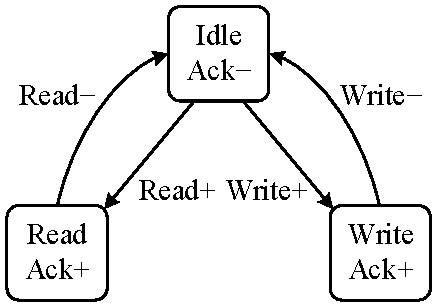
\includegraphics[scale=0.5]{figs/StateDiagramTopV4}
    \caption{State diagram (top level).}
    \label{fig:StateDiagramTop}
\end{figure}
\begin{figure*}[ht]
    \centering
    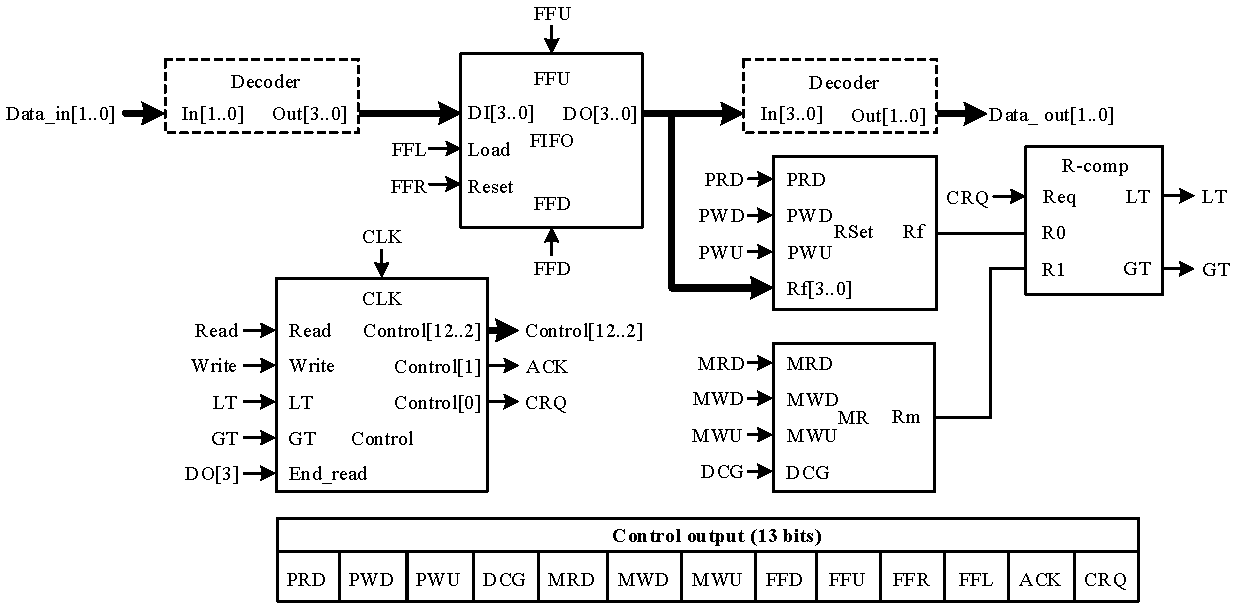
\includegraphics[scale=0.7]{figs/SystemV5}
    \caption{Overall circuit.}
    \label{fig:System}
\end{figure*}
\begin{table}[ht]
   \centering
   \caption{Signal Description.}
   \label{tab:SignalDescription}
   \begin{tabular}{| l | l |}
       \hline
       \thead{Name}& 
       \thead{Description}\\
       \hline
       \hline
       CLK	& Control clock \\
       \hline
       Read	& Request read data \\
       \hline
%        Clear	& Request clear data \\
%        \hline
       Write	& Request write data \\
       \hline
       LT		& Comparison result: G\textsubscript{m} < G\textsubscript{f} (less than)\\
       \hline
       GT		& Comparison result: G\textsubscript{m} $\geq$ G\textsubscript{f} (greater than or equal to)\\
       \hline  
       End\_read & Terminate data reading operation \\
	   \hline
       PRD   	& Enable padding for reading \\
	   \hline
	   PWD  	& Enable padding for writing down \\
       \hline
       PWU   	& Enable padding for writing up \\
       \hline
       DCG 		& Discharge memristor \\
       \hline
       MRD		& Enable memristor for reading \\
       \hline
       MWD		& Enable memristor for writing down \\
       \hline
       MWU		& Enable memristor for writing up \\
       \hline
       FFD		& Shift FIFO down \\
       \hline
       FFU		& Shift FIFO up \\
       \hline
       FFR		& Reset FIFO \\
       \hline
       FFL		& Load FIFO \\
       \hline
       ACK		& Control acknowledge \\
       \hline
       CRQ		& Request resistance comparison \\
       \hline
%        DO		& Data out \\
%        \hline       
   \end{tabular}
\end{table}
% \begin{table}[ht]
%    \centering
%    \caption{Decoder input and output.}
%    \label{tab:DecoderInputAndOutput}
%    \begin{tabular}{| c | c |}
%        \hline
%        \thead{Data}& 
%        \thead{One-hot code}
% %        \thead{Selected}&
% %        \thead{Resistance}
%        \\
% %        \thead{In[2..0]} & \thead{Out[2..0]} & \thead{resistor} & \thead{(K$\Omega$)} \\
%        \hline
%        \hline
%        00   	& 0001 \\
% 	   \hline
%        01  		& 0010 \\
%        \hline
%        10		& 0100 \\
%        \hline
%        11		& 1000 \\
%        \hline
%    \end{tabular}
% \end{table}
\subsection{Resistance comparator and its metastability issue}
\label{subsec:ResistanceComparatorAndItsMetastabilityIssue}
The resistance comparator is shown in Fig.~\ref{fig:ComparatorWithBooster}. The idea of this comparator is to \textit{compare the currents that relate to the resistors}. 
When the request signal Req is 0, the transistors MN1 and MN3 pull the outputs q0 and q1 to ground which represents the result of 00 (standby). The resistance comparison is performed when Req is 1. In this case, MN1 and MN3 are OFF and MP1 and MP4 inject the currents that are inversely proportional to the values of the connected resistors to nodes q0 and q1. At these nodes, both currents are against each other and logic 1 is indicated the winner node while logic 0 remains in the loser node. Note that, to describe the result in terms of conductance which is applied throughout of this text, the winner node implies its conductance has a larger value than the other.
\begin{figure}[ht]
    \centering
    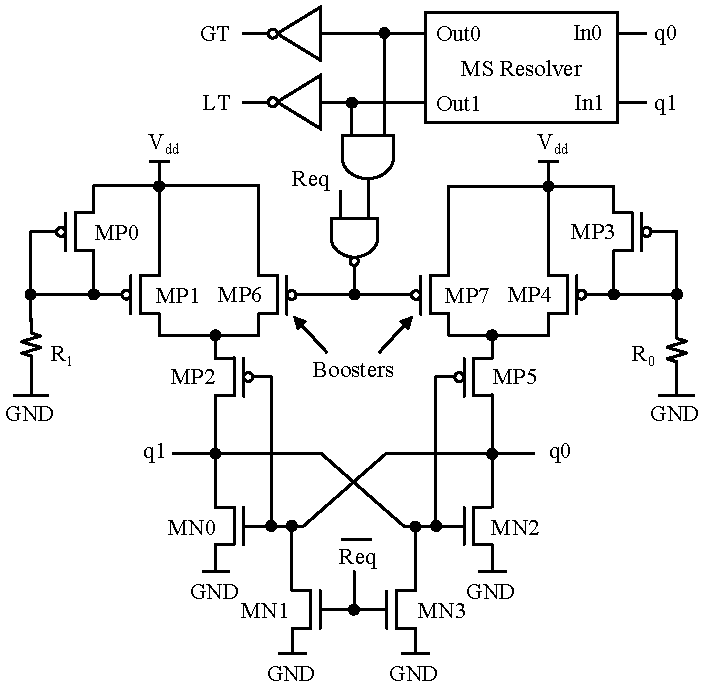
\includegraphics[scale=0.6]{figs/ComparatorWithBoosterV4}
    \caption{Resistance comparator.}
    \label{fig:ComparatorWithBooster}
\end{figure}

The metastability resolver (MSR) is attached to the outputs q0 and q1 to filter the metastability state the circuit enters during the resistance comparison. Its circuit and simulation result are illustrated in Fig.~\ref{fig:MSR} and Fig.~\ref{fig:ComparatorMs} respectively. When the comparator is on standby, logic 0 presented at both inputs (In0 and In1) turn on both PMOSs so that both outputs (Out0 and Out1) are connected to V\textsubscript{dd} (logic 1). These outputs are the same when the metastability exists because PMOSs and NMOSs are still ON and OFF respectively. Finally, when the differential logic inputs arrive, either MP0 and MN1 or MP1 and MN0 are ON accordingly and the inputs propagate to the outputs. In conclusion, the inserted MSR can prevent the failure in the rest of the system that is caused by this ambiguous metastable state. Note that, for simulation shown in Fig.~\ref{fig:ComparatorMs}, both resistor sizes are chosen the same, in order to implement the worst case scenario where the comparator takes the longest time to generate the result and the resistance of 300K$\Omega$ is selected as it is the maximum value of the selected memristor. Table~\ref{tab:ResultDescriptionOfTheResistanceComparator} describes the signal at each node in regard to the comparison result.

\begin{figure}[ht]
    \centering
    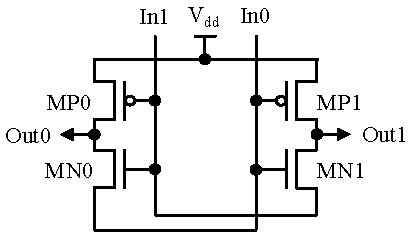
\includegraphics[scale=0.6]{figs/MSR}
    \caption{Metastability resolver (MSR).}
    \label{fig:MSR}
\end{figure}
\begin{figure}[ht]
    \centering
    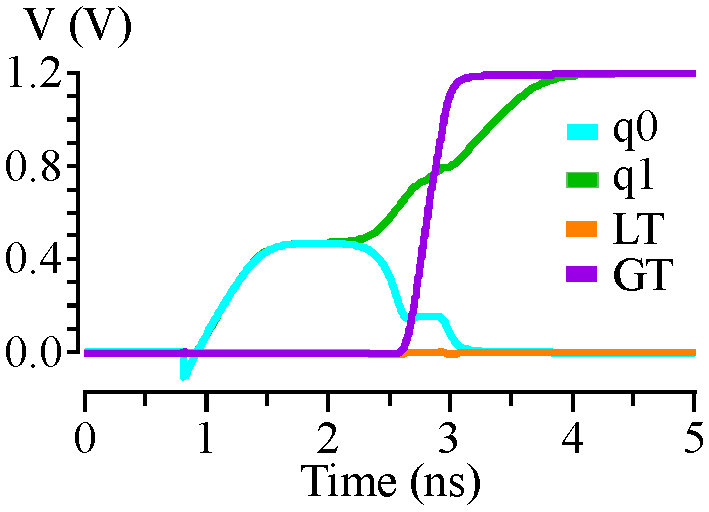
\includegraphics[scale=0.4]{figs/ComparatorMsV4}
    \caption{The outputs of the resistance comparator (q0 and q1) and MSR (LT and GT) when R\textsubscript{0}=R\textsubscript{1}=300K$\Omega$.}
    \label{fig:ComparatorMs}
\end{figure}
\begin{table}[ht]
   \centering
   \caption{Result Description of the Resistance Comparator.}
   \label{tab:ResultDescriptionOfTheResistanceComparator}
   \begin{tabular}{| c | c | c |}
       \hline
       \multirow{2}{*}{\thead{Result}}& 
       \multicolumn{2}{|c|}{\thead{Signal}}\\
       \cline{2-3}
       &\thead{q1, q0}&
       \thead{GT, LT}      
       \\
       \hline
       \hline
       Standby   						& 0, 0 & 1, 1 \\
	   \hline
       G\textsubscript{m} $\geq$ G\textsubscript{f} (R\textsubscript{m} < R\textsubscript{f})   	& 1, 0 & 1, 0 \\
	   \hline
	   G\textsubscript{m} < G\textsubscript{f} (R\textsubscript{m} $\geq$ R\textsubscript{f})   				& 0, 1 & 0, 1 \\
       \hline
   \end{tabular}
\end{table}

Lastly, the boosters \cite{Zhou-2006-ISVLSI} (MP6 and MP7 in Fig.~\ref{fig:ComparatorWithBooster}) are added to the circuit to improve the computation speed. They are ON and equally inject additional currents to q0 and q1 when Req arrives but the outputs are still invalid (both Out0 and Out1 are 1). From Fig.~\ref{fig:ComparatorDelayVsResistance}, suppose both resistances are the same to yield the worst case delay, the time the comparator without boosters takes to produce valid outputs increases with the values of the resistors. This is because the generated currents are small when the resistances are high. With the boosters, the delay increases gradually and it is smaller than that of the circuit without boosters even at the small resistance comparison (1K$\Omega$ range). However, these boosters trade timing improvement with accuracy. The graph in Fig.~\ref{fig:ComparatorResolution} shows the comparator without boosters provides better resolution when high resistance comparison is performed because, at high resistances, the current flows from MP1 and MP7 are very small while the large currents from the boosters fulfill the parasitic capacitances at q0 and q1 quickly. So the charge difference is insufficient for providing correct outputs. Note that, the simulation results of LT=0 and GT=1 are always given when the resistive difference is smaller than the safe resolution.

\begin{figure}[ht]
    \centering
    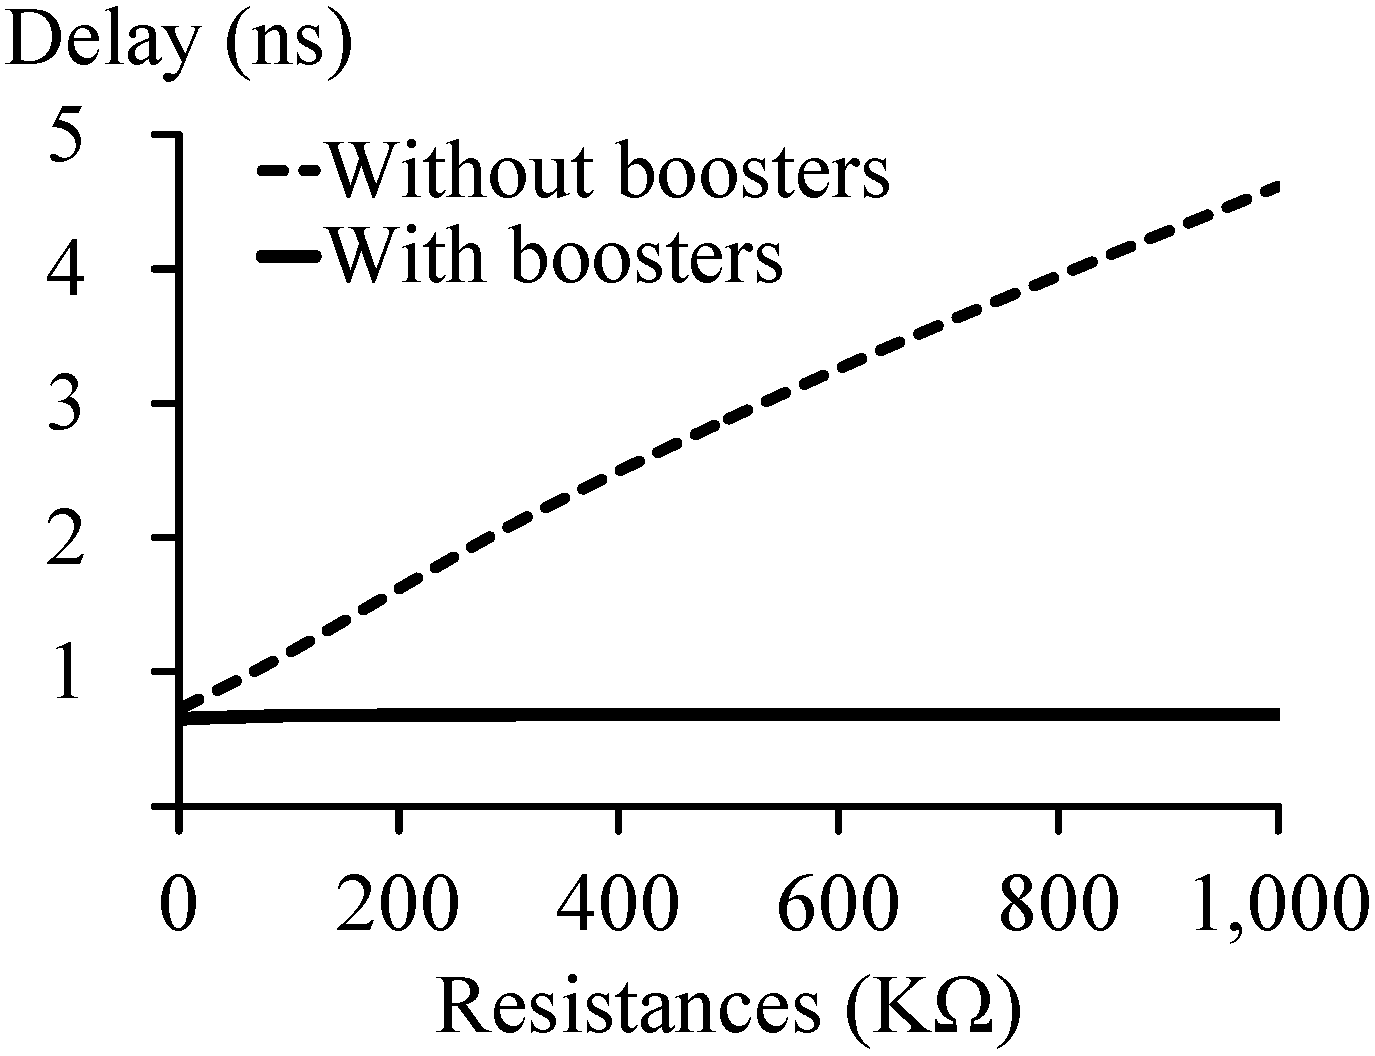
\includegraphics[scale=0.2]{figs/ComparatorDelayVsResistance}
    \caption{Delays of the resistance comparator with (solid) and without (dash) boosters (R\textsubscript{0}=R\textsubscript{1}=[1, 1,000]K$\Omega$).}
    \label{fig:ComparatorDelayVsResistance}
\end{figure}
\begin{figure}[ht]
    \centering
    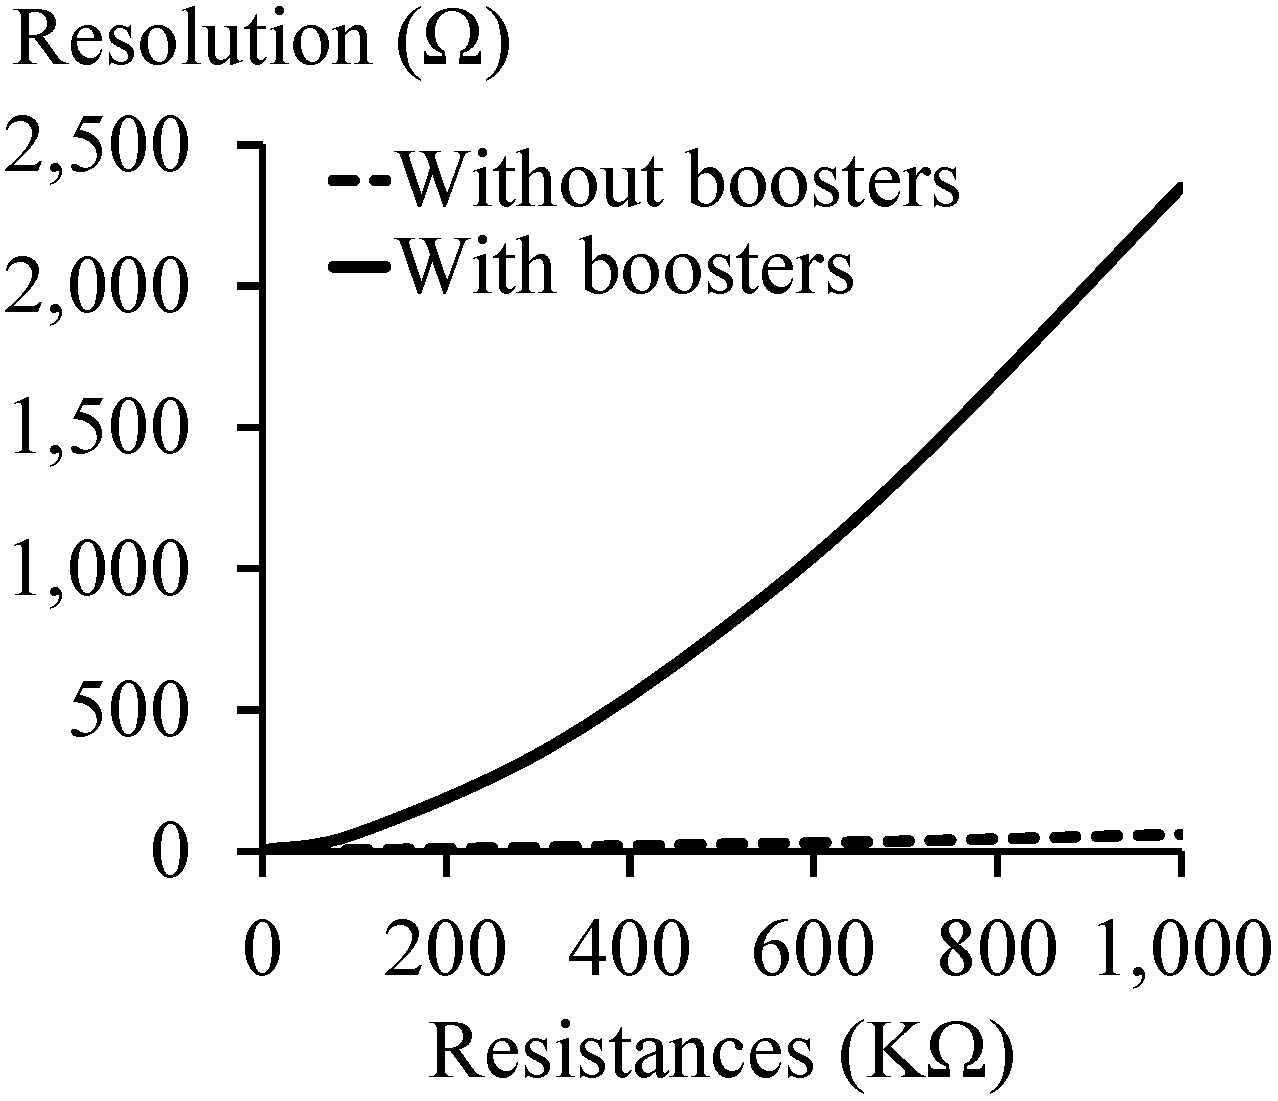
\includegraphics[scale=0.2]{figs/ComparatorResolution}
    \caption{Resolutions of the resistance comparator with (solid) and without (dash) boosters (R\textsubscript{0}=R\textsubscript{1}=[1, 1,000]K$\Omega$).}
    \label{fig:ComparatorResolution}
\end{figure}

\subsection{Memristor access mechanism and reference resistor set}
\label{subsec:MemristorAccessMechanismAndReferenceResistorSet}
To battle against the PVT variations where the memristance can be shifted unexpectedly, the resistive buffers (paddings) between each data region are needed. Therefore, the memristor access mechanism for each operating sequence (in term of conductance) and the corresponding reference resistor set are designed as shown in Fig.~\ref{fig:MemristorAccess} and Fig.~\ref{fig:RSet}. Note that all reference resistances (R\textsubscript{f}) are complied with the condition: R\textsubscript{f0}~$>$~R\textsubscript{f1}~$>$~R\textsubscript{f2}~$>$~R\textsubscript{f3} (G\textsubscript{f0}~$<$~G\textsubscript{f1}~$<$~G\textsubscript{f2}~$<$~G\textsubscript{f3}). Note that the inverters that complement the signals Rf0 to Rf3 are not included in the figure.

\begin{figure}[ht]
    \centering
    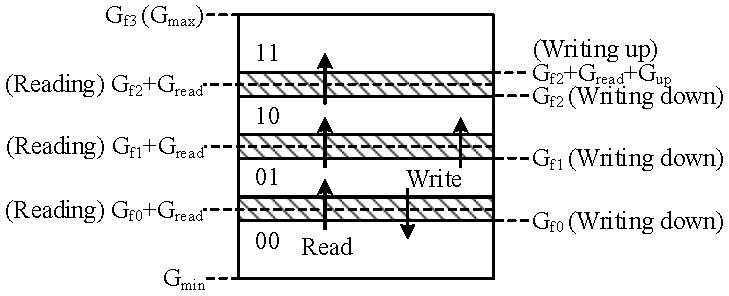
\includegraphics[scale=0.65]{figs/MemristorAccessV5}
    \caption{Memristor access diagram.}
    \label{fig:MemristorAccess}
\end{figure}
\begin{figure}[ht]
    \centering
    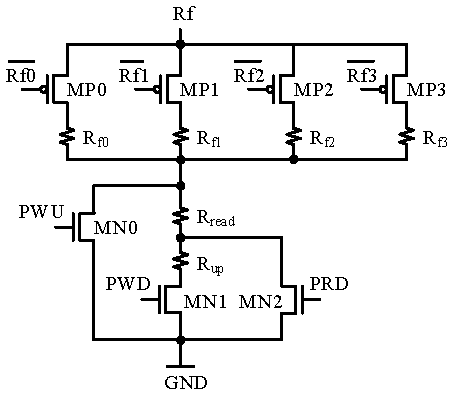
\includegraphics[scale=0.7]{figs/RSetV5}
    \caption{Reference resistor set circuit.}
    \label{fig:RSet}
\end{figure}

In data reading, the sequence starts from sending PRD signal to turn on MN2 to bypass R\textsubscript{up} and sending Rf0 signal to connect R\textsubscript{f0}, which is the lowest conductance, to Rf node. This results in the lowest reading conductance (G\textsubscript{f0}$+$G\textsubscript{read}) which is located in the middle of the lowest buffer (the patterned box). In conductance comparison, if the memristor conductance is lower than the formed conductance, the data is recognized as 00. Otherwise, the next conductance level which is higher than the first one is established (G\textsubscript{f1}$+$G\textsubscript{read}). This time, data 01 is sent out if the memristor conductance is lower or the next reading level (G\textsubscript{f2}$+$G\textsubscript{read}) is constructed otherwise. At this stage, data 10 is recognized if the memristor conductance is lower, otherwise, data is sent out as 11 instead. Note that the last reference conductance is not necessary in reading because the last comparison can distinguish between 10 and 11. The proper implementation of the controller in defined in Section~\ref{subsec:ReadMode}.

There are two types of writing: write down and write up. %In both types, the memristance is shifted between data regions without the need for erasure. 
In write down operation, PWD is sent to omit R\textsubscript{read} and R\textsubscript{up}, and one of Rf signals selects a reference resistor depending on the data in FIFO. This forms only G\textsubscript{f} as a reference conductance which locates the bottom of the selected buffer. Then, the memristor is tuned down until its conductance is lower than the reference one. In write up operation, PWU is 1 instead of PWD and the FIFO is shifted down one step to select the conductance that is lower than the current one. This yield the reference conductance of G\textsubscript{f(n-1)}$+$G\textsubscript{read}$+$G\textsubscript{up}. For example, in writing data 10, the FIFO will be loaded with data 0100 (Table~\ref{tab:DataRepresentation}) and then it is shifted down to 0010 to select G\textsubscript{f1}. Thereafter, the memristor is tuned up until the its conductance is higher than G\textsubscript{f1}$+$G\textsubscript{read}$+$G\textsubscript{up}. Full controller implementation for this operation in described in Section~\ref{subsec:WriteMode}.

Based on the specified memristance range in Table~\ref{tab:DataRepresentation}, all resistors in RSet module have been defined as listed in Table~\ref{tab:ResistorListForRSet}. Note that R\textsubscript{f} means the selected one from the available reference resistor (R\textsubscript{f0} or R\textsubscript{f1} or R\textsubscript{f2} or R\textsubscript{f3}) and both resistances R\textsubscript{read} and R\textsubscript{up} are 3K$\Omega$. Due to zero resistance of R\textsubscript{f3}, it will be replaced by a connection wire.
\begin{table}[ht]
   \centering
   \caption{Resistor List for RSet.}
   \label{tab:ResistorListForRSet}
   \begin{tabular}{| l | l | r |}
       \hline
       \multirow{2}{*}{\thead{Signal}}&
       \thead{Selected}& 
       \thead{Total resistance}\\
       & \thead{resistor} & \thead{(K$\Omega$)} \\
       \hline
       \hline
       Rf0	&	R\textsubscript{f0}	&	167 \\
       \hline
       Rf1	&	R\textsubscript{f1}	&	147 \\
       \hline
       Rf2	&	R\textsubscript{f2}	&	127 \\
       \hline
       Rf3	&	R\textsubscript{f3}	&	0 \\
       \hline       
       PRD	&	R\textsubscript{read}  & R\textsubscript{f} + 3 \\
	   \hline
	   PWD	&	R\textsubscript{read}, R\textsubscript{up}   & R\textsubscript{f} + 6 \\
       \hline
       PWU	&	None  & R\textsubscript{f} \\
       \hline
   \end{tabular}
\end{table}
\begin{table}[ht]
   \centering
   \caption{FIFO module operation.}
   \label{tab:FIFOModuleOperation}
   \begin{tabular}{| c | c | c | c | l | c | c |}
       \hline
       \multicolumn{4}{| c |}{\thead{Signal}}& 
       \multirow{2}{*}{\thead{Description}}&
       \multirow{2}{*}{\thead{DO[3..0]}}&
       \multirow{2}{*}{\thead{Selected}}\\
       \cline{1-4}
       \thead{FFR} & \thead{FFU} & \thead{FFD} & \thead{FFL} &&&\thead{resistor}\\
       \hline
       \hline
       1&0&0&0	& Reset (default) 	& 0001 		& R\textsubscript{f0} \\
       \hline
       0&1&0&0	& First shift up	& 0010		& R\textsubscript{f1} \\
       \hline
       0&1&0&0	& Second shift up	& 0100		& R\textsubscript{f2} \\
       \hline
       0&1&0&0	& Third shift up	& 1000		& Bypass\\
       \hline
       0&0&1&0	& Shift down		& 0100		& R\textsubscript{f2}\\
       \hline       
       0&0&0&1	& Load 				& DI[3..0] 	& Depend\\
       %& R\textsubscript{f0}/R\textsubscript{f1}/R\textsubscript{f2} \\
       \hline       
   \end{tabular}
\end{table}
\subsection{FIFO}
\label{subsec:FIFO}
This 4-bits FIFO receives the one-hot data from the decoder and receives four control signals (FFD, FFU, FFR and FFL) from the controller. The one-hot outputs of this FIFO are connected to RSet module to select a reference resistor in RSet. Four functions of this FIFO are listed in Table~\ref{tab:FIFOModuleOperation}. The reset function is invoked (FFR=1) to clears all internal data to 0001 when the system finishes a particular operation and wants to return to the idle state. By clearing data to 0001, the lowest reference conductance (G\textsubscript{f0}) is always selected by default. In data reading mode, therefore, the controller can start comparison without the need for shifting. The shifting up is required only when the comparison result shows the memristor conductance is higher than the reference one. This can be done by sending FFU signal as logic 1 to CLK terminal. As a result, the higher reference conductance is selected. This shifting continues until the controller finishes obtaining the stored data. For data writing, the controller will send FFL signal as logic 1 to load this FIFO with the decoded data and this data will select a particular reference conductance. Then, the controller will shift the FIFO down (sending FFD as 1) when it enters write up sequence.

\subsection{Memristor and interfacing circuit}
\label{subsec:MemristorAndInterfacingCircuit}
This circuit provides four functions: memristor reading, writing down, writing up and discharge which are one-hot controlled by MRD, MWD, MWU and DCG respectively as shown in Fig.~\ref{fig:MemristorInterfacing}. Note that the inverters that generate the complement signals are not included in the figure. 

In data reading, MP3 and MN0 are ON by logic 1 at MRD. This will connect the memristor to the resistance comparator. MWD and MWU are used to tune the memristance down and up by connecting power supply to the memristor terminals but in opposite direction. Discharging is necessary before read-after-write, which happens in both write up and down sequences, is performed. Once logic 1 is applied at DCG, the charge at both memristor terminal are flushed while the node Rm is fully charged by power supply. Without discharging, the remaining charges from memristance tuning stage will interfere the voltage at Rm and cause an incorrect result. 
\begin{figure}[ht]
    \centering
    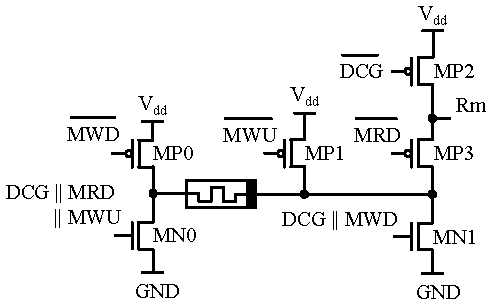
\includegraphics[scale=0.7]{figs/MemristorInterfacingCircuitV3}
    \caption{Memristor interfacing circuit.}
    \label{fig:MemristorInterfacing}
\end{figure}
\section{Synchronous Controller}
\label{sec:SynchronousController}
\subsection{Read mode}
\label{subsec:ReadMode}
The idea of data reading is to compare the conductance between the memristor and each reference resistor in RSet which is selected from the lowest to the highest conductance by one-hot code from the FIFO as described in Table~\ref{tab:FIFOModuleOperation}. 
From the state diagram in Fig.~\ref{fig:StateDiagramRead}, the controller perform the first reading iteration without shifting FIFO because it already selects the lowest reference conductance (G\textsubscript{f0}) by default. It only enables the read padding resistor and the memristor (PRD$+$ and MRD$+$) and then starts the comparison by sending CRQ$+$ signal to the comparator. In returned result consideration, if LT$+$ is observed, it means the memristor conductance is less than the lowest reference conductance. Based on data representation in Table~\ref{tab:DataRepresentation}, therefore, the data is recognized as 00 and the controller steps to Send\_ack. Otherwise (GT$+$: greater than), the controller shifts the FIFO up (FFU$+$, one-hot:0010) to connect G\textsubscript{f1} to the comparator and start comparison again. At this time, the controller goes to Send\_ack and the read out data is 01 if LT$+$ is inspected or the controller prepares for the third comparison instead. Again, the FIFO is shifted up (FFU$+$, one-hot:0100) so that G\textsubscript{f2} is attached to the comparator. When the comparison is performed, the controller moves to Send\_ack and the data is read as 10 if LT$+$ is detected. Otherwise, it shifts the FIFO up to 1000 by sending FFU$+$. At this point D[3] of the FIFO, which is fed back to the controller at End\_FIFO pin (Fig.~\ref{fig:System}), is detected as 1. Therefore, the controller switches to Send\_ack instead and the output data from FIFO is encoded as 11.
\begin{figure}[t]
    \centering
    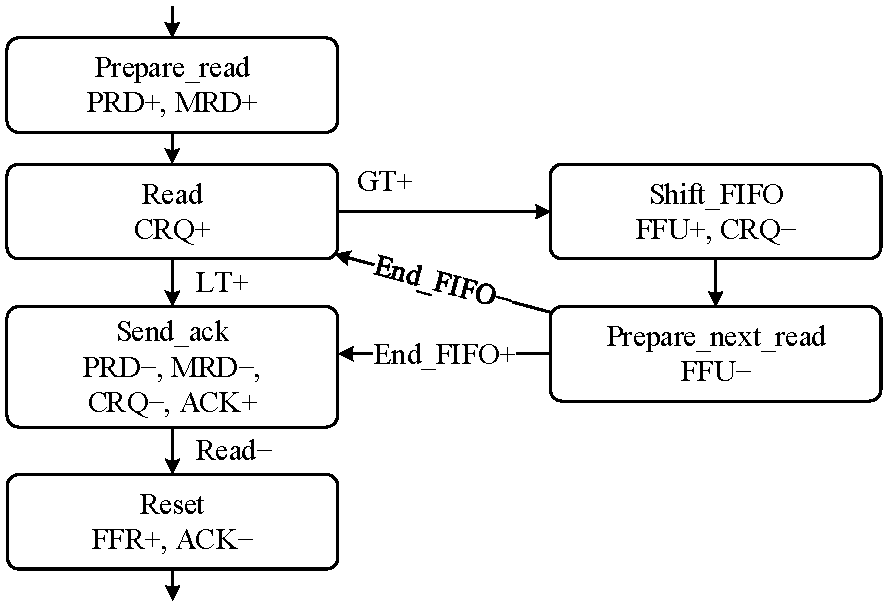
\includegraphics[scale=0.5]{figs/StateDiagramReadV5}
    \caption{State diagram (read data).}
    \label{fig:StateDiagramRead}
\end{figure}
\begin{figure}[ht]
    \centering
    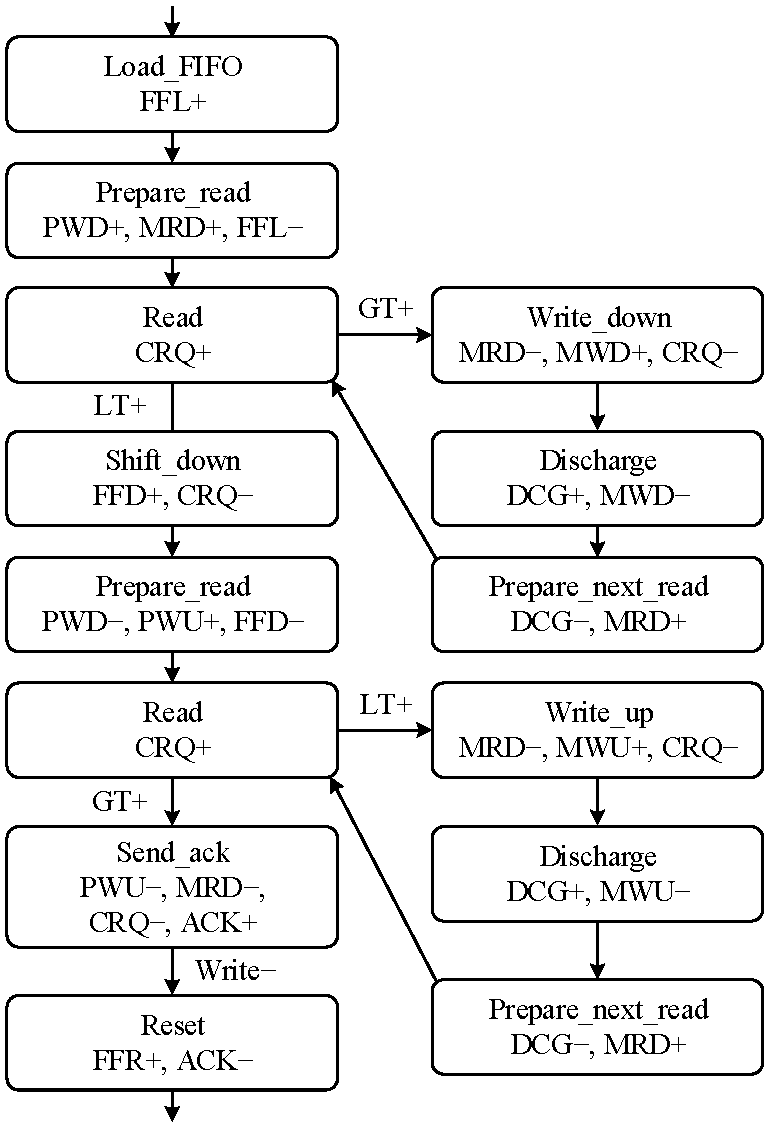
\includegraphics[scale=0.5]{figs/StateDiagramWriteV5}
    \caption{State diagram (write data).}
    \label{fig:StateDiagramWrite}
\end{figure}
\begin{figure}[ht]
    \centering
    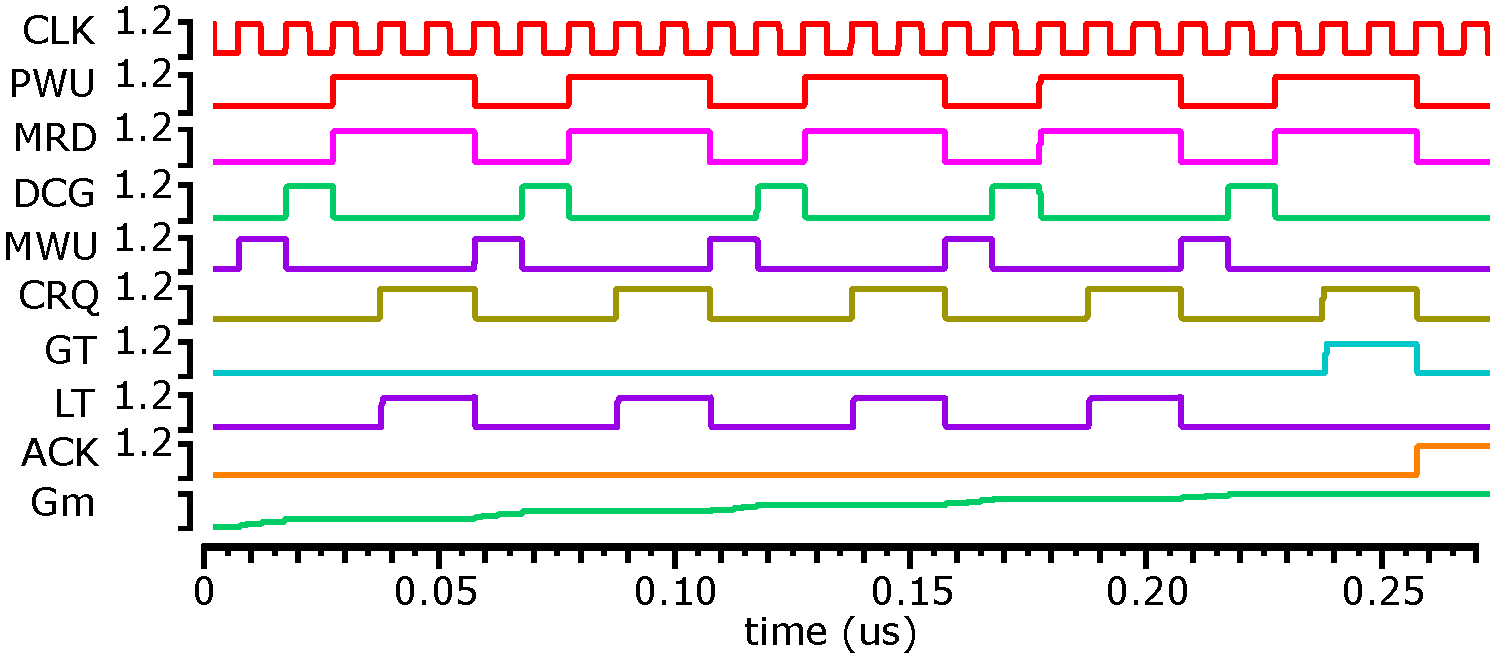
\includegraphics[scale=0.33]{figs/SimWrite}
    \caption{Simulation result (write up from 00 to 11).}
    \label{fig:SimWrite}
\end{figure}
\subsection{Write mode}
\label{subsec:WriteMode}
Initially, the operation is assumed as writing down (new data is lower than the current one). The operation starts by sending FFL$+$ to load the FIFO with the decoded data input. Then, PWD$+$ and MRD$+$ are sent to address a reference conductance at the bottom of the buffer (Section~\ref{subsec:MemristorAccessMechanismAndReferenceResistorSet}) and to enable the memristor for reading respectively. Next, the comparison takes place (CRQ$+$) and the write down operation is confirmed if the memristor conductance is higher than the reference one (GT$+$). Otherwise (LT$+$), the operation switches to write up. Once write down operation is confirmed, the memristor conductance is tuned down for 10ns by signal MWD$+$ and then the charge between its terminals are emptied by signal DCG$+$. Next, MRD$+$ is sent out to prepare the memristor for the next reading. Subsequently, the comparison is performed again and the write down loop continues until the memristor conductance is less than the reference one. 

Whether the controller entered the write down loop or not, it steps to write up preparation stage where the FIFO is shifted down (FFD$+$) to select the lower buffer and PWU$+$ is sent to address the maximum conductance of such buffer (Section~\ref{subsec:MemristorAccessMechanismAndReferenceResistorSet}). Then, the comparison takes place and the controller enters the write up loop, which is similar to the write down one except MWU$+$ is sent out instead, if it receives LT$+$ as a result or it goes to Send\_ack state to finish the operation otherwise (GT$+$). The simulation result for writing data from 00 to 11 is depicted in Fig.~\ref{fig:SimWrite}. It can be seen that the memristor conductance (Gm) is increased when MWU is active and the tuning continues until the comparison result GT is 1.

\section{Asynchronous Controller}
\label{sec:AsynchronousController}

The synchronous controller in the previous section is converted to an asynchronous version which is formally specified by the signal transition graph~(STG)~\cite{Chu-1987-PhD} in Fig.~\ref{fig:MainControlSTG}. It represents the read and write modes of the controller operation that are selected by READ$+$ and WRITE$+$ signals, respectively.

\begin{figure*}[ht]
    \centering
    \begin{subfigure}[b]{\textwidth}
        \centering
        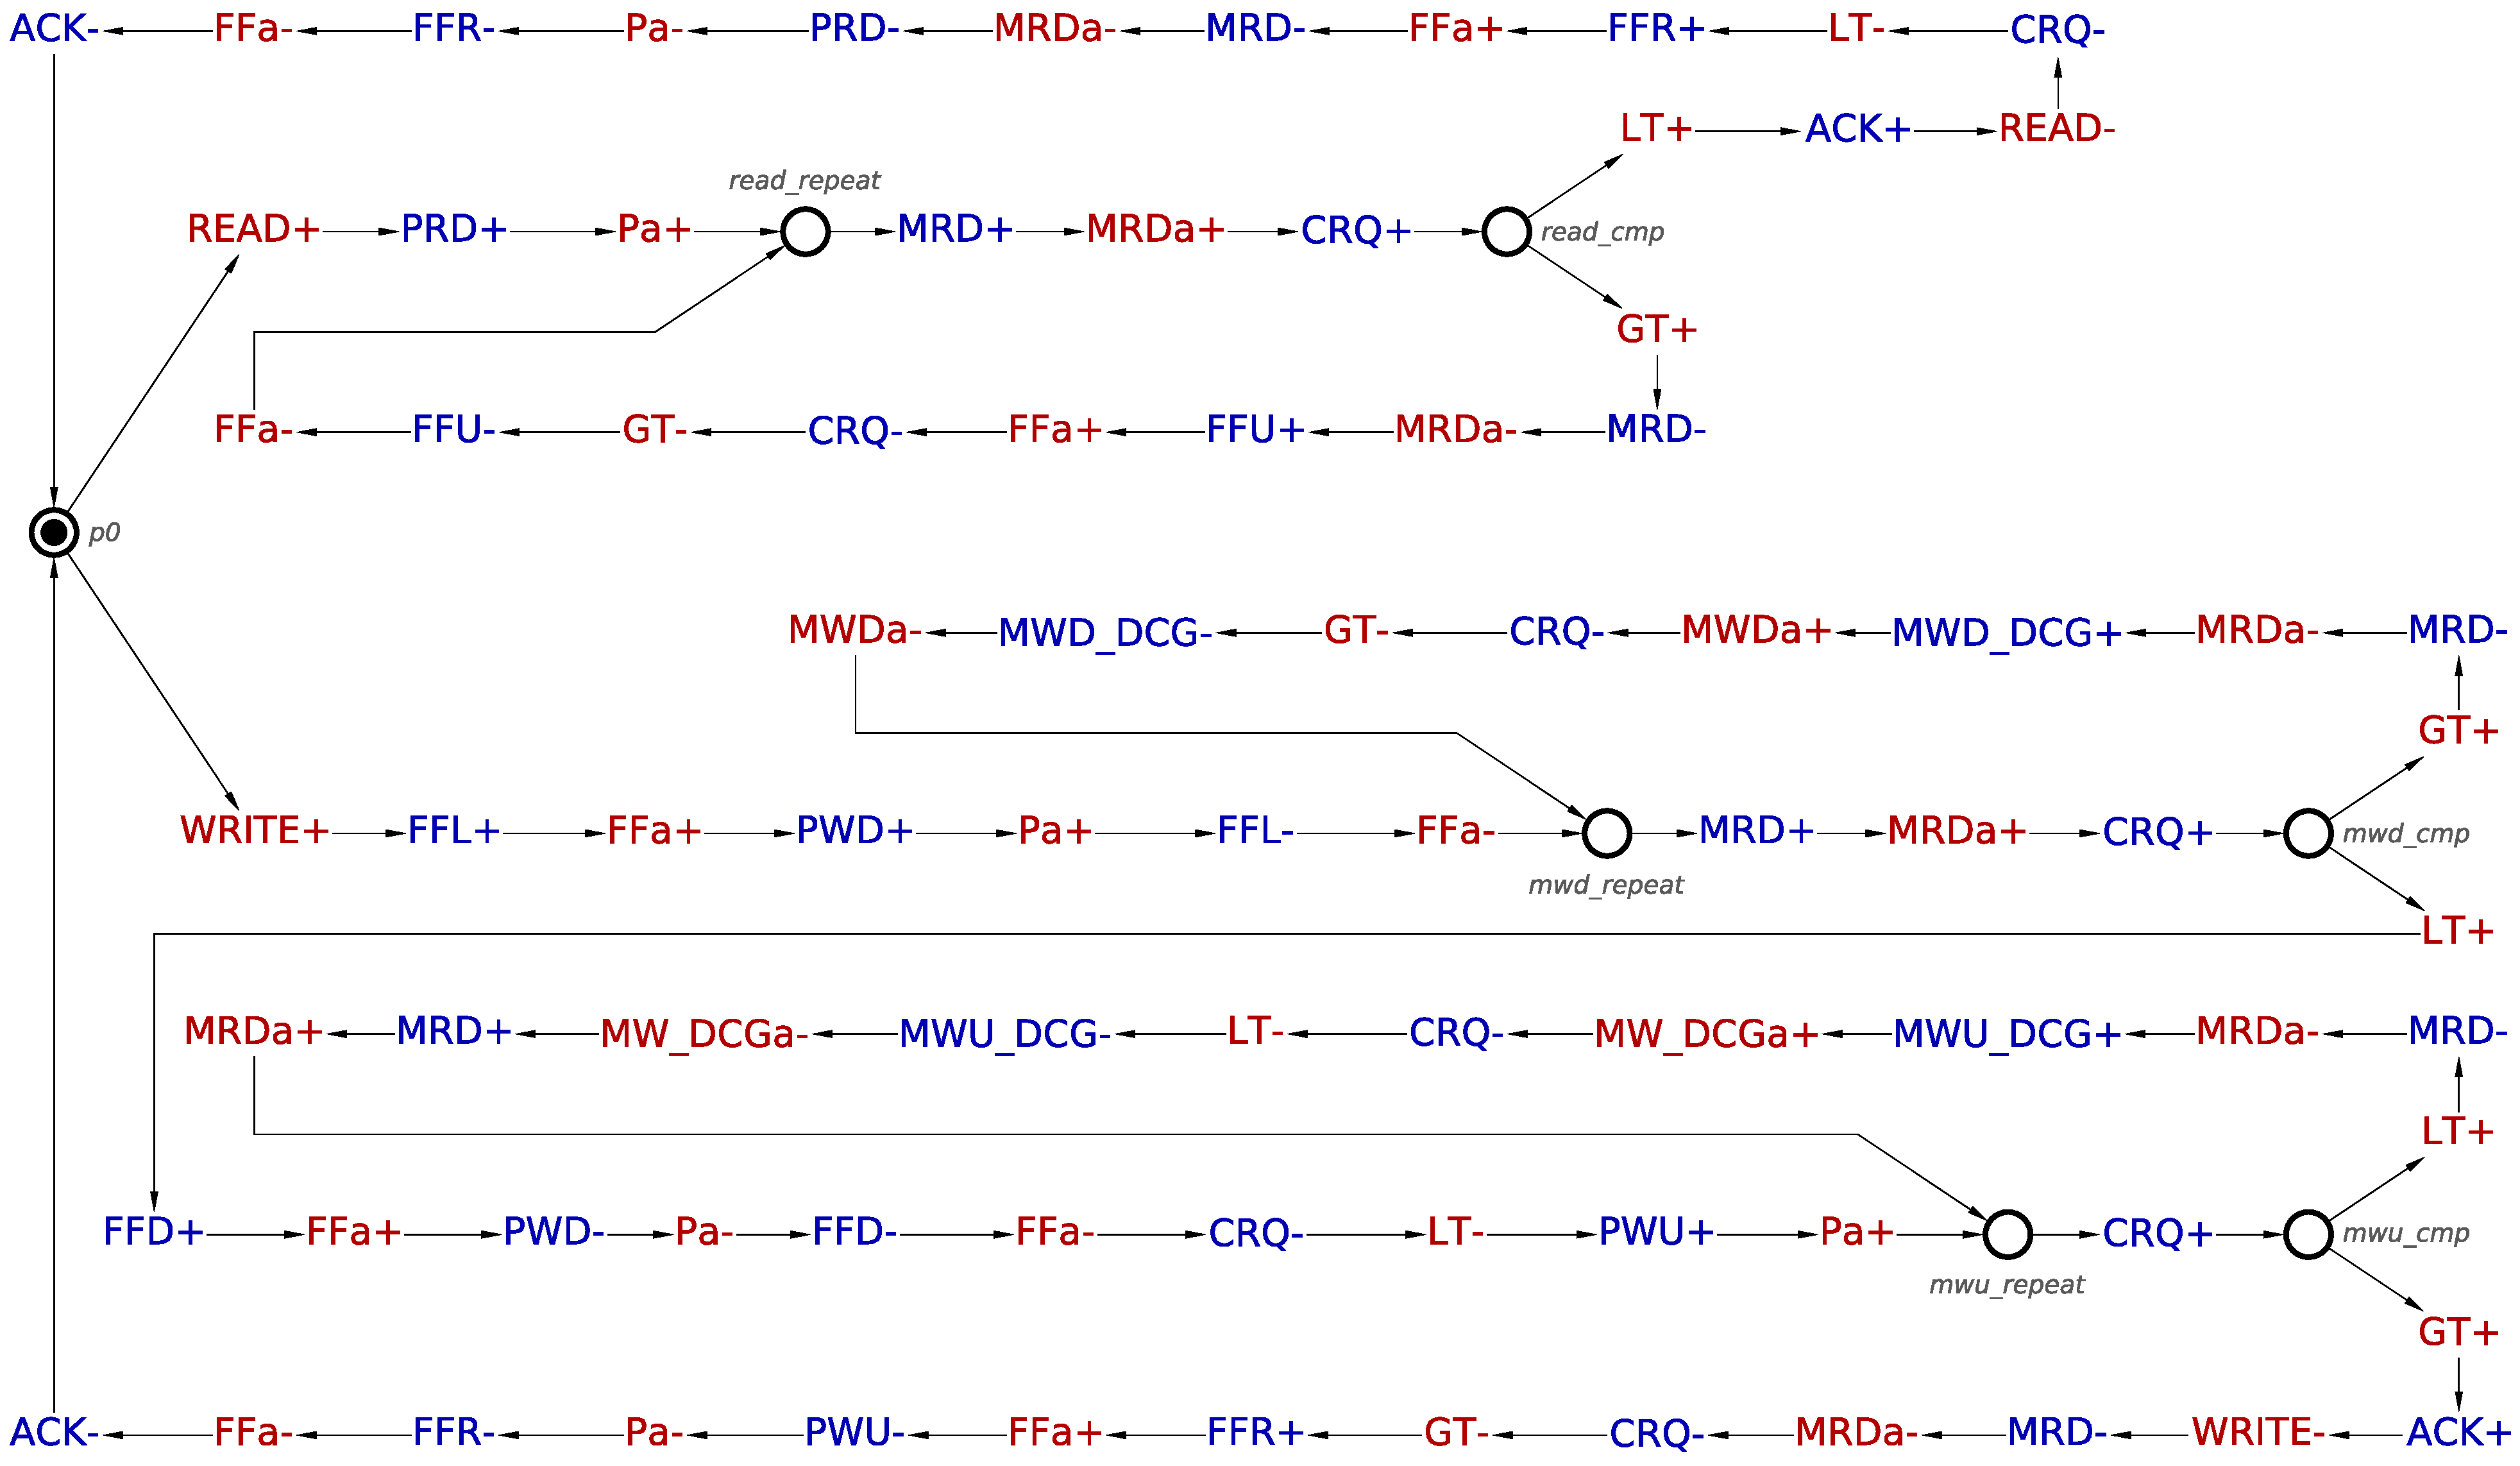
\includegraphics[scale=0.2]{figs/main_ctrl_stg}
        \caption{Main controller.}
        \label{fig:MainControlSTG}
    \end{subfigure}
	\vspace{10pt}

    \begin{subfigure}[b]{\textwidth}
        \centering
        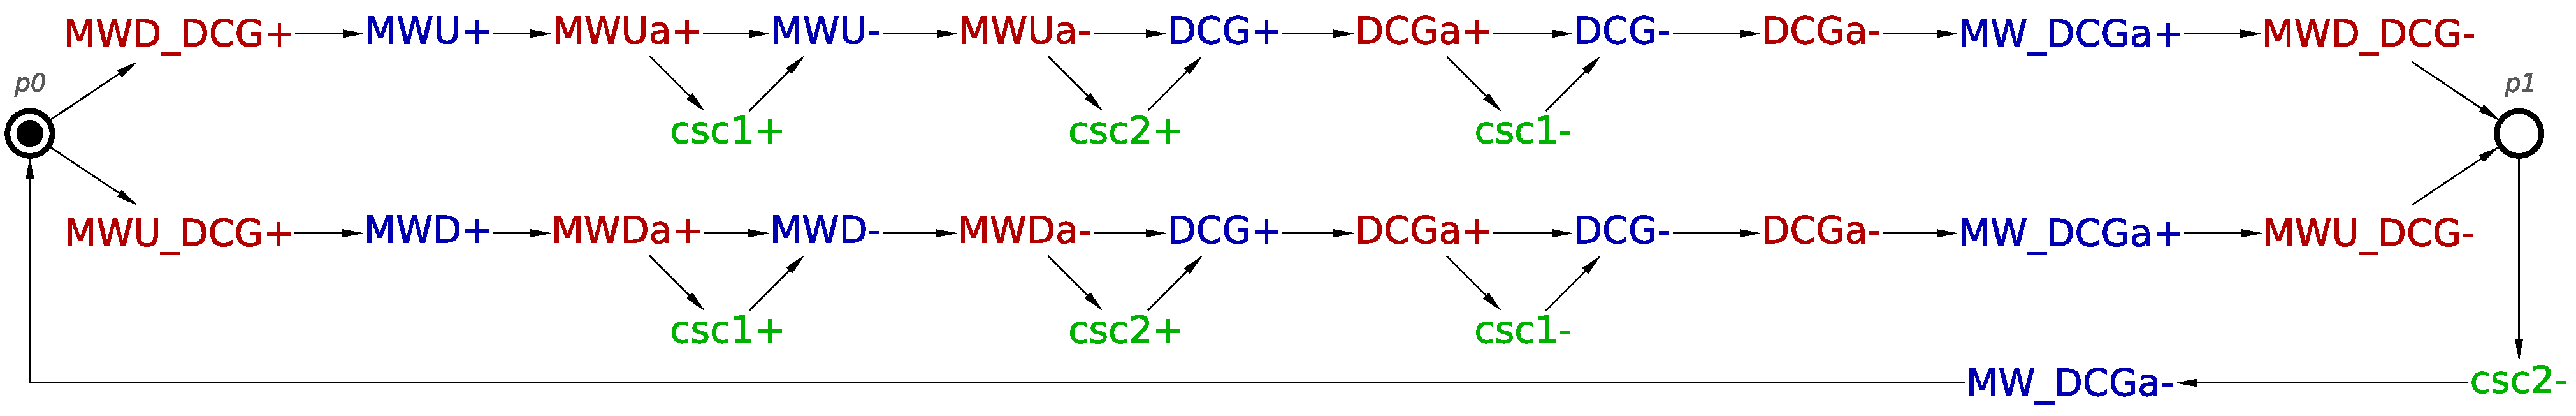
\includegraphics[scale=0.2]{figs/write_discharge_csc_stg}
        \caption{Write and discharge module.}
        \label{fig:WriteDischargeSTG}
    \end{subfigure}
    \caption{STG specification of the controller.}
    \label{fig:ControlSTG}
\end{figure*}

In the read mode the read-padding is applied via PRD/PRDa handshake, the memristor state is fetched by MRD/MRDa handshake and compared against a reference resistor. The reference register is selected by the one-hot code in the FIFO that is iteratively shifted up by the FFU/FFa handshake. When the reference conductance becomes grater than the memristor conductance, the reading completion is indicated by ACK$+$ and the FIFO holds a one-hot code that represents the read value.  On the exit from the reading mode the FIFO is reset to the initial state via FFR/FFa handshake.

In the write mode the one-hot code for the desired value is loaded in the FIFO via FFL/FFa handshake. The one-hot code selects the reference resistor that is compared against the current conductance of the memristor. If the reference is greater~(less) than the memristor conductance, then the write-down~(write-up) pulses are applied until the memristor conductance becomes less~(greater) than the reference. Note that write-down and write-up paddings are selected via PWD/Pa and PWU/Pa handshakes, respectively.

To reduce complexity of the controller, the write-up (MWU/MWUa handshake) and write-down (MWD/MWDa handshake) functions are factored out in a separate \textsf{write\_discharge} module, as shown in Fig.~\ref{fig:ControllerTopCircuit}. Its STG specification is shown in Fig.~\ref{fig:WriteDischargeSTG} -- in addition to the writing pulses this component also discharges the parasitic capacitors via DCG/DCGa handshake before the state of memristor can be fetched. Additional signals csc1 and csc2 were inserted to resolve complete state coding conflicts.

\begin{figure}[h]
    \centering
    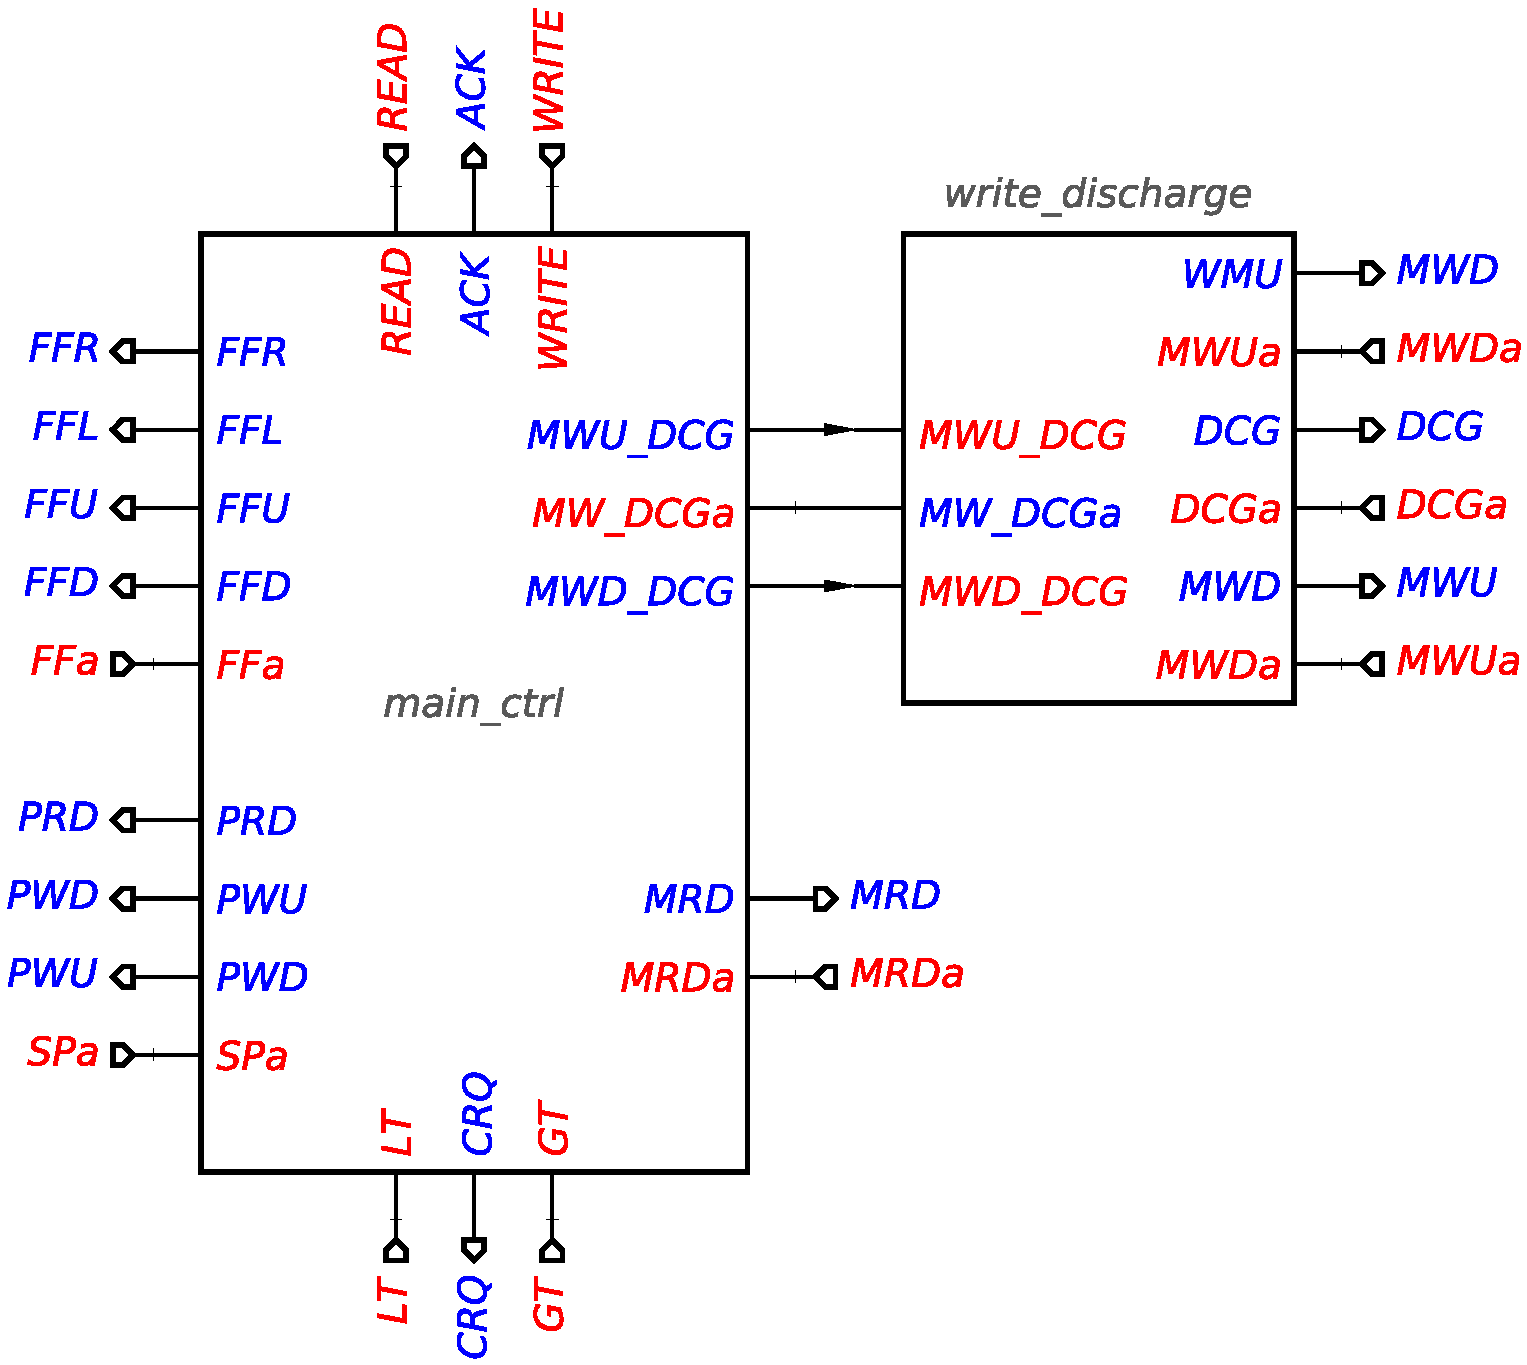
\includegraphics[scale=0.3]{figs/control_circuit}
    \caption{Signal transition graph for write and discharge.}
    \label{fig:ControllerTopCircuit}
\end{figure}

The STG specifications for the asynchronous controller have been developed and formally verified in Workcraft software~\cite{Sokolov-2016-book-Workcraft}. The STGs are confirmed to be consistent, free of deadlocks, output persistent, exhibit complete state coding and can be synthesized into the speed-independent circuits~\cite{Muller-1959-ts}. The complex-gate synthesis has been successful and produced the following equations:\\
\footnotesize
\textsf{[ACK] = (GT PWU + LT READ) + ACK (Pa + FFa);}\\
\textsf{[CRQ] = (FFa' GT MWDa' PWU' + MRDa (Pa PWU + READ + PWD))\\
\hspace*{25pt}+ CRQ (GT' MRDa' MW\_DCGa' + MRDa FFa);}\\
\textsf{[FFD] = (LT PWD) + FFD Pa;}\\
\textsf{[FFL] = MRD' Pa' WRITE;}\\
\textsf{[FFR] = LT' GT' Pa ACK;}\\
\textsf{[FFU] = GT MRDa' PRD;}\\
\textsf{[MRD] = (GT' PWU' FFa' Pa MWDa' + LT' PWU WRITE MW\_DCGa'\\
\hspace*{25pt}+ FFD) + MRD (PWD' PRD' PWU');}\\
\textsf{[MWD\_DCG] = GT MRDa' PWD;}\\
\textsf{[MWU\_DCG] = LT MRDa';}\\
\textsf{[PRD] = READ + PRD MRDa;}\\
\textsf{[PWD] = (MRD' FFa WRITE) + PWD FFa';}\\
\textsf{[PWU] = (LT' MRD PWD' PRD') + PWU FFa';}\\
\textsf{[DCG] = csc1 csc2;}\\
\textsf{[MWD] = csc1' csc2' MWU\_DCG;}\\
\textsf{[MWU] = csc1' csc2' MWD\_DCG;}\\
\textsf{[MW\_DCGa] = DCGa' csc1' csc2;}\\
\textsf{[csc1] = (MWUa + MWDa) + csc1 DCGa';}\\
\textsf{[csc2] = (csc1 MWDa' MWUa') + csc2 (MWD\_DCG + MWU\_DCG);}\\
\normalsize

Unfortunately the technology mapping of the main controller into UMC 65nm gate library failed both with MPSat~\cite{Khomenko-2009-TR-MPSat} and Petrify~\cite{Cortadella-1997-Petrify} backends. The problem has been reported to the developers of MPSat and was confirmed to be a bug in the tool that is relatively easy to fix.

While the technology mapping issue prevented us from including the simulation results for the asynchronous controller, we expect it to exhibit significantly lower latency -- just few gate delays, as opposed to the clock cycle period in synchronous design.

We will include this simulation results in the final version of the paper. If an updated version of MPSat is released by then we will stick with the speed-independent implementation of the asynchronous controller. As a backup solution we plan to drop the speed-independent requirement  and manually decompose the complex gate equations under fundamental mode timing assumption.

% \subsection{Synchronous controller}
% \label{subsec:SynchronousController}
% \subsection{Asynchronous controller}
% \label{subsec:AsynchronousController}
% \section{Simulation result}
% \label{sec:SimulationResult}


\section{Conclusion}
\label{sec:Conclusion}

This paper presents an approach in designing memristor-based multi-bits memory cell~(3MCell). The advantages of this design are only one supply voltage requirement, high data capacity support and PVT variation tolerance. Our resistance comparator design operates at high precision to provide a high data capacity. Moreover, a metastability resolver is applied to fix the metastability state the comparator enters during the comparison. To improve robustness to PVT variations, the resistive buffers are provided by the reference resistor set~(RSet). Finally, the controller is developed in both synchronous and asynchronous styles. Implementation of the asynchronous controller in UMC 65nm gate library and its simulation in the system context is the work in progress.

\bibliographystyle{IEEEtran}
\bibliography{refs}

\end{document}
